\subsection{Station Software}
While the figure of the overall architecture gives a nice look at the system, the station component has its own architecture as well, which can be seen in \figref{fig:stationarch}. In this figure, as in the previous, the arrows represent flow of information.

\begin{figure}[h]
	\centering
	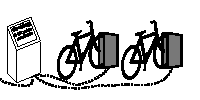
\includegraphics[trim=2cm 9.5cm 0cm 3cm, clip, scale=0.6]{design/station}
	\caption{Station software architecture}\label{fig:stationarch}
\end{figure}

In the station software, the station is the main part and also the one that contains the UI. 
This part is responsible for all contact with the user at the station and is the one that is connected to the hardware.
\textit{TCPlistener} is a thread that listens for messages from the bigger system and stores these messages as a \textit{networkData} object, and tells this object to perform the action the message contains.
The \textit{networkData} object then either adds a booking to the local database corresponding to the information the object contains, or removes a booking with the ID it received.
The \textit{LockManager} is also a thread, this one is responsible for locking a bicycle when a booking is close to its start time and unlocking said bicycle again if the booking's start time is exceeded by a certain limit.
The last class is the \textit{ServiceThreads} which is also running in a separate thread.
This thread is responsible for reporting changes at the station, which are stored in the \textit{toReport} attribute.
As soon as there is something in the \textit{toReport} list, the thread will try to report it to the online interface, repeating until it succeeds in getting its message through.